\section{Annexes}
\subsection{Avis personnels et problèmes rencontrés}
\paragraph{Tristan :}
\begin{itemize}
\item[$\bullet$]Communication (qui fait quoi, quand et pourquoi\dots )
\item[$\bullet$]Conflits SVN
\item[$\bullet$]Implémentation pascal linux = caca
\end{itemize}
\paragraph{Rémi :}
\begin{itemize}
\item[$\bullet$] Les autres ont rien foutus
\end{itemize}
\paragraph{Victor :}
\begin{itemize}
\item Idem
\end{itemize}

\paragraph{Théo :}
\begin{itemize}
\item niah
\end{itemize}

\newpage
\subsection{Diagrammes de classes}

\begin{center}
\begin{figure}[h]
\begin{center}
\scalebox{0.5}[0.42]{\includegraphics*{../images/UML.jpeg}}
\end{center}
\caption{Diagramme de classe utilisé pour notre projet}
\end{figure}
\end{center}
%% Graphic for TeX using PGF
% Title: /home/blackout/Documents/Sources/2010_pascal_moteur_2D/trunk/doc/Diagramme UML.dia
% Creator: Dia v0.97.1
% CreationDate: Sat May 28 23:45:59 2011
% For: blackout
% \usepackage{tikz}
% The following commands are not supported in PSTricks at present
% We define them conditionally, so when they are implemented,
% this pgf file will use them.
\ifx\du\undefined
  \newlength{\du}
\fi
\setlength{\du}{15\unitlength}
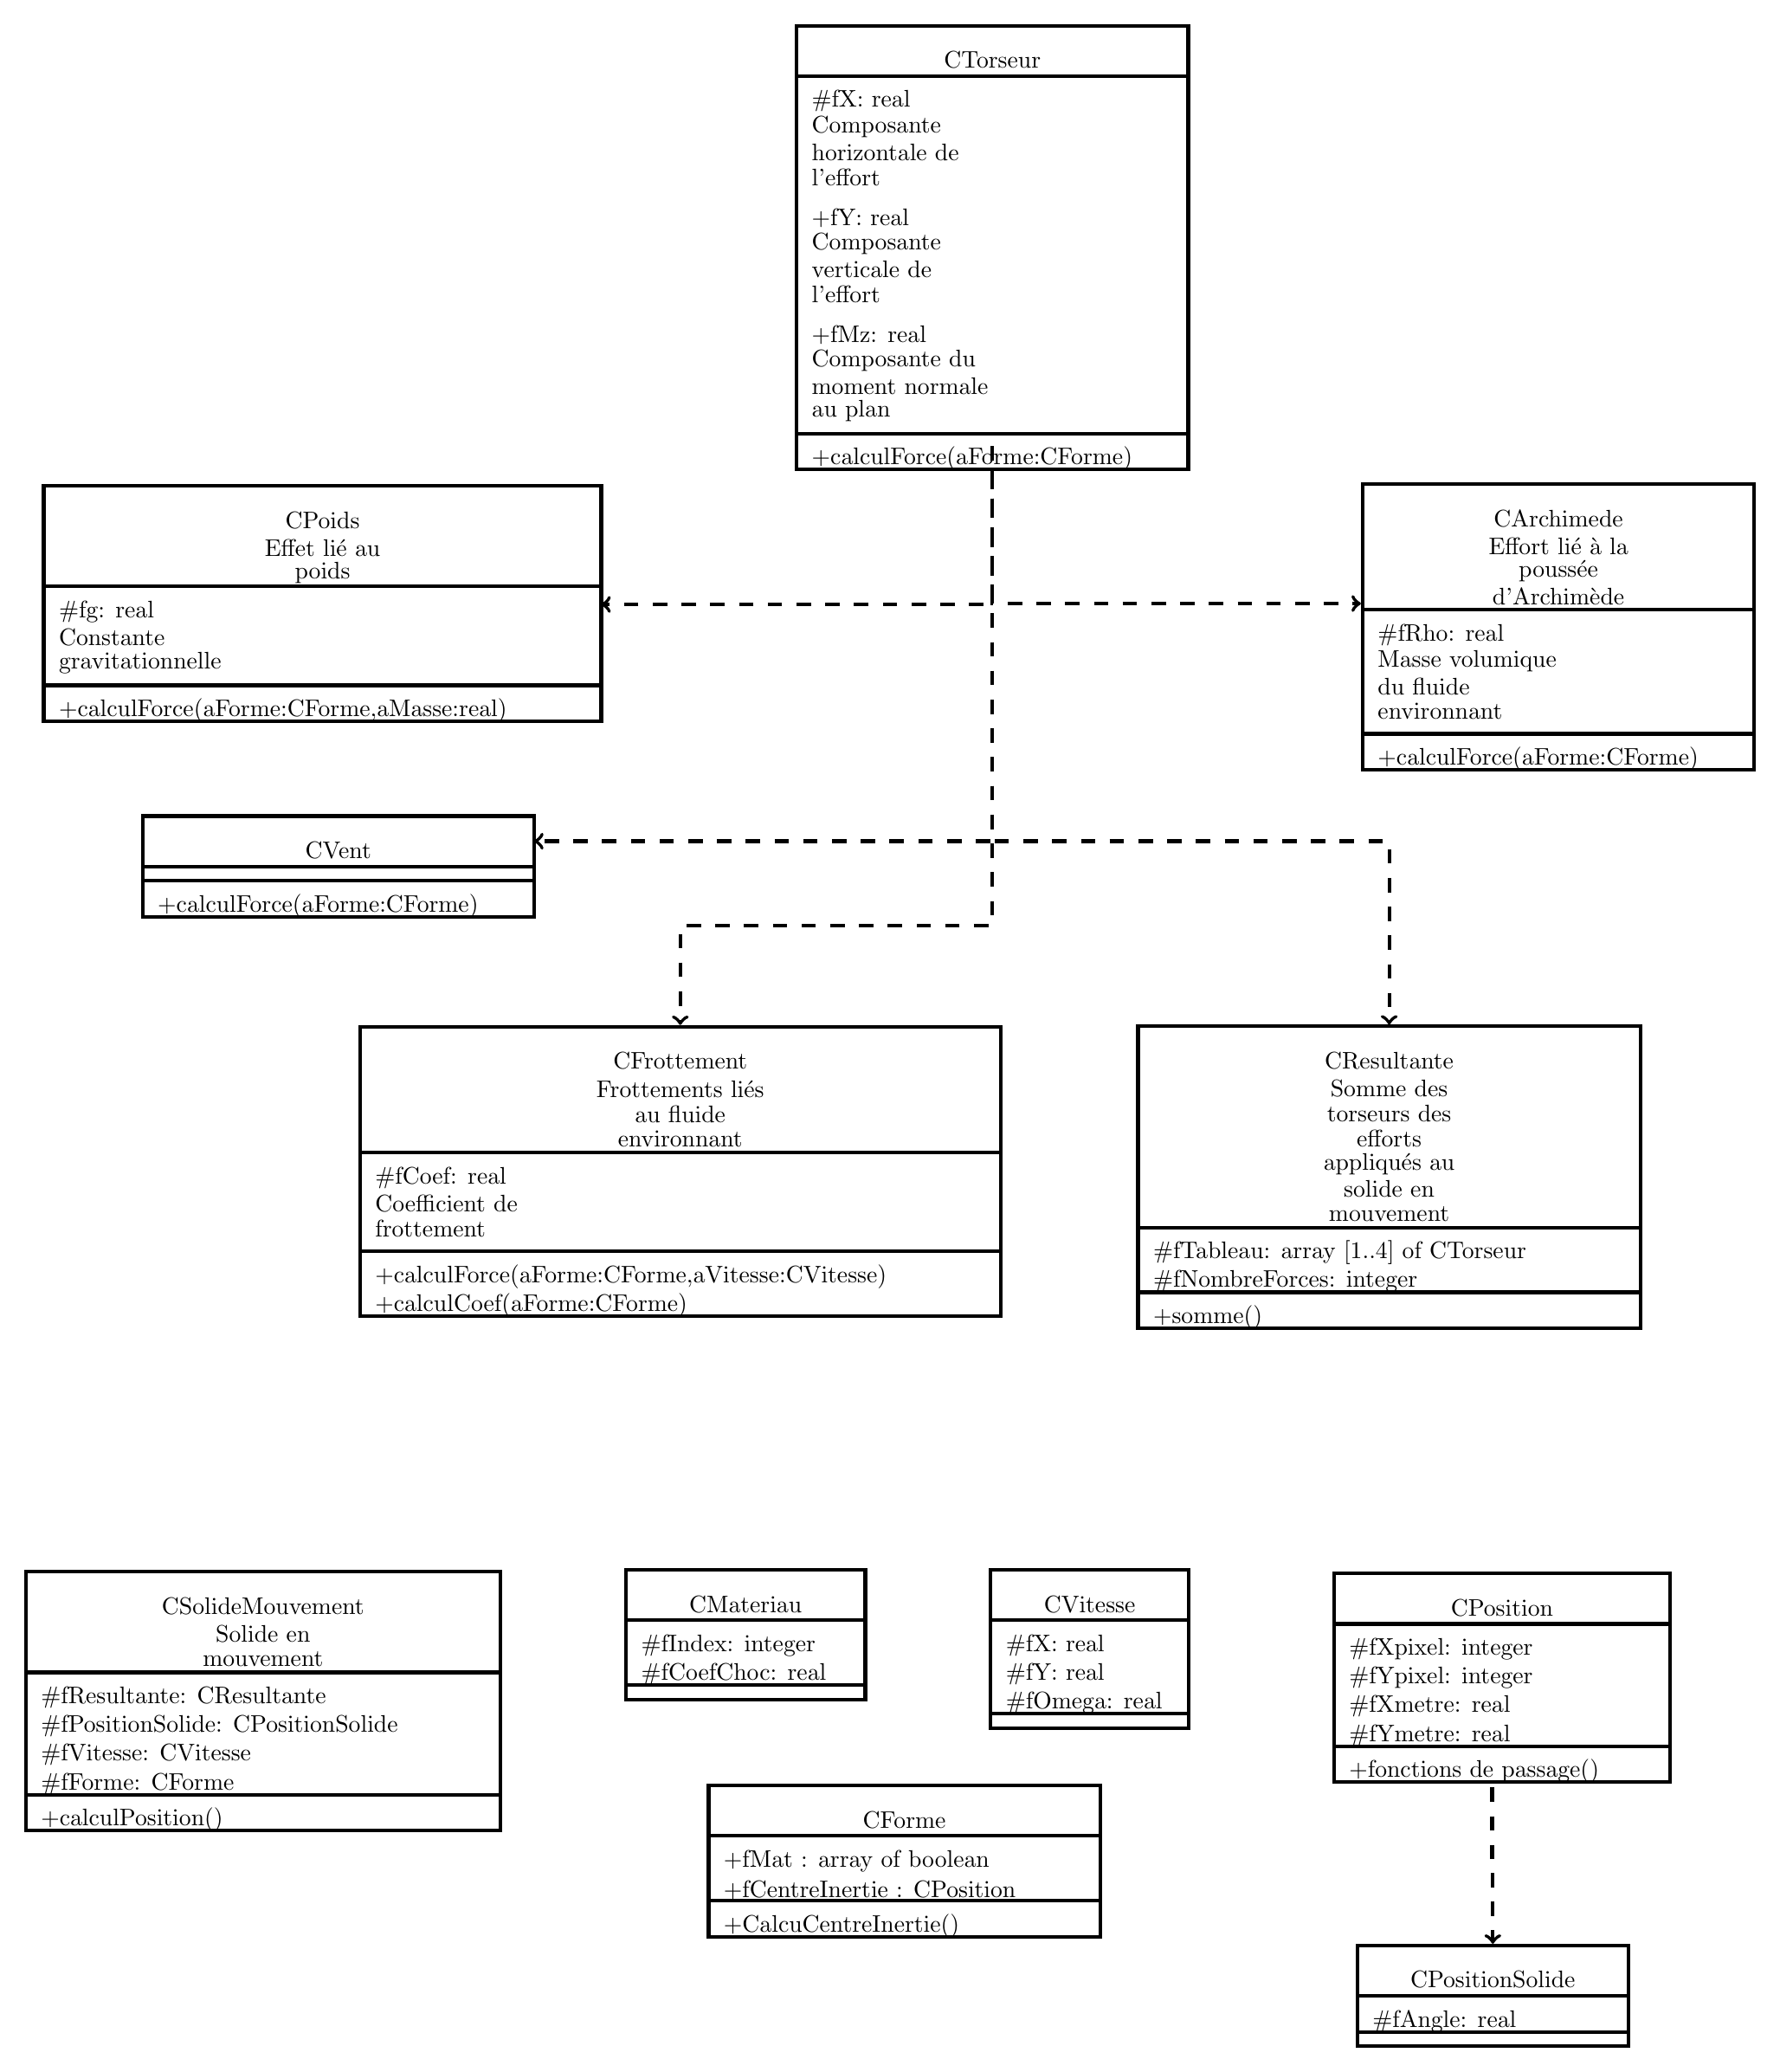
\begin{tikzpicture}
\pgftransformxscale{1.000000}
\pgftransformyscale{-1.000000}
\definecolor{dialinecolor}{rgb}{0.000000, 0.000000, 0.000000}
\pgfsetstrokecolor{dialinecolor}
\definecolor{dialinecolor}{rgb}{1.000000, 1.000000, 1.000000}
\pgfsetfillcolor{dialinecolor}
\pgfsetlinewidth{0.100000\du}
\pgfsetdash{}{0pt}
\definecolor{dialinecolor}{rgb}{1.000000, 1.000000, 1.000000}
\pgfsetfillcolor{dialinecolor}
\fill (31.550000\du,-8.750000\du)--(31.550000\du,-7.350000\du)--(42.445000\du,-7.350000\du)--(42.445000\du,-8.750000\du)--cycle;
\definecolor{dialinecolor}{rgb}{0.000000, 0.000000, 0.000000}
\pgfsetstrokecolor{dialinecolor}
\draw (31.550000\du,-8.750000\du)--(31.550000\du,-7.350000\du)--(42.445000\du,-7.350000\du)--(42.445000\du,-8.750000\du)--cycle;
% setfont left to latex
\definecolor{dialinecolor}{rgb}{0.000000, 0.000000, 0.000000}
\pgfsetstrokecolor{dialinecolor}
\node at (36.997500\du,-7.800000\du){CTorseur};
\definecolor{dialinecolor}{rgb}{1.000000, 1.000000, 1.000000}
\pgfsetfillcolor{dialinecolor}
\fill (31.550000\du,-7.350000\du)--(31.550000\du,2.600000\du)--(42.445000\du,2.600000\du)--(42.445000\du,-7.350000\du)--cycle;
\definecolor{dialinecolor}{rgb}{0.000000, 0.000000, 0.000000}
\pgfsetstrokecolor{dialinecolor}
\draw (31.550000\du,-7.350000\du)--(31.550000\du,2.600000\du)--(42.445000\du,2.600000\du)--(42.445000\du,-7.350000\du)--cycle;
% setfont left to latex
\definecolor{dialinecolor}{rgb}{0.000000, 0.000000, 0.000000}
\pgfsetstrokecolor{dialinecolor}
\node[anchor=west] at (31.700000\du,-6.650000\du){\#fX: real};
% setfont left to latex
\definecolor{dialinecolor}{rgb}{0.000000, 0.000000, 0.000000}
\pgfsetstrokecolor{dialinecolor}
\node[anchor=west] at (31.700000\du,-5.925000\du){Composante};
\definecolor{dialinecolor}{rgb}{0.000000, 0.000000, 0.000000}
\pgfsetstrokecolor{dialinecolor}
\node[anchor=west] at (31.700000\du,-5.225000\du){horizontale de};
\definecolor{dialinecolor}{rgb}{0.000000, 0.000000, 0.000000}
\pgfsetstrokecolor{dialinecolor}
\node[anchor=west] at (31.700000\du,-4.525000\du){l'effort};
% setfont left to latex
\definecolor{dialinecolor}{rgb}{0.000000, 0.000000, 0.000000}
\pgfsetstrokecolor{dialinecolor}
\node[anchor=west] at (31.700000\du,-3.400000\du){+fY: real};
% setfont left to latex
\definecolor{dialinecolor}{rgb}{0.000000, 0.000000, 0.000000}
\pgfsetstrokecolor{dialinecolor}
\node[anchor=west] at (31.700000\du,-2.675000\du){Composante};
\definecolor{dialinecolor}{rgb}{0.000000, 0.000000, 0.000000}
\pgfsetstrokecolor{dialinecolor}
\node[anchor=west] at (31.700000\du,-1.975000\du){verticale de};
\definecolor{dialinecolor}{rgb}{0.000000, 0.000000, 0.000000}
\pgfsetstrokecolor{dialinecolor}
\node[anchor=west] at (31.700000\du,-1.275000\du){l'effort};
% setfont left to latex
\definecolor{dialinecolor}{rgb}{0.000000, 0.000000, 0.000000}
\pgfsetstrokecolor{dialinecolor}
\node[anchor=west] at (31.700000\du,-0.150000\du){+fMz: real};
% setfont left to latex
\definecolor{dialinecolor}{rgb}{0.000000, 0.000000, 0.000000}
\pgfsetstrokecolor{dialinecolor}
\node[anchor=west] at (31.700000\du,0.575000\du){Composante du};
\definecolor{dialinecolor}{rgb}{0.000000, 0.000000, 0.000000}
\pgfsetstrokecolor{dialinecolor}
\node[anchor=west] at (31.700000\du,1.275000\du){moment normale};
\definecolor{dialinecolor}{rgb}{0.000000, 0.000000, 0.000000}
\pgfsetstrokecolor{dialinecolor}
\node[anchor=west] at (31.700000\du,1.975000\du){au plan};
\definecolor{dialinecolor}{rgb}{1.000000, 1.000000, 1.000000}
\pgfsetfillcolor{dialinecolor}
\fill (31.550000\du,2.600000\du)--(31.550000\du,3.600000\du)--(42.445000\du,3.600000\du)--(42.445000\du,2.600000\du)--cycle;
\definecolor{dialinecolor}{rgb}{0.000000, 0.000000, 0.000000}
\pgfsetstrokecolor{dialinecolor}
\draw (31.550000\du,2.600000\du)--(31.550000\du,3.600000\du)--(42.445000\du,3.600000\du)--(42.445000\du,2.600000\du)--cycle;
% setfont left to latex
\definecolor{dialinecolor}{rgb}{0.000000, 0.000000, 0.000000}
\pgfsetstrokecolor{dialinecolor}
\node[anchor=west] at (31.700000\du,3.300000\du){+calculForce(aForme:CForme)};
\pgfsetlinewidth{0.100000\du}
\pgfsetdash{}{0pt}
\definecolor{dialinecolor}{rgb}{1.000000, 1.000000, 1.000000}
\pgfsetfillcolor{dialinecolor}
\fill (10.600000\du,4.050000\du)--(10.600000\du,6.850000\du)--(26.115000\du,6.850000\du)--(26.115000\du,4.050000\du)--cycle;
\definecolor{dialinecolor}{rgb}{0.000000, 0.000000, 0.000000}
\pgfsetstrokecolor{dialinecolor}
\draw (10.600000\du,4.050000\du)--(10.600000\du,6.850000\du)--(26.115000\du,6.850000\du)--(26.115000\du,4.050000\du)--cycle;
% setfont left to latex
\definecolor{dialinecolor}{rgb}{0.000000, 0.000000, 0.000000}
\pgfsetstrokecolor{dialinecolor}
\node at (18.357500\du,5.000000\du){CPoids};
% setfont left to latex
\definecolor{dialinecolor}{rgb}{0.000000, 0.000000, 0.000000}
\pgfsetstrokecolor{dialinecolor}
\node at (18.357500\du,5.775000\du){Effet lié au};
\definecolor{dialinecolor}{rgb}{0.000000, 0.000000, 0.000000}
\pgfsetstrokecolor{dialinecolor}
\node at (18.357500\du,6.475000\du){poids};
\definecolor{dialinecolor}{rgb}{1.000000, 1.000000, 1.000000}
\pgfsetfillcolor{dialinecolor}
\fill (10.600000\du,6.850000\du)--(10.600000\du,9.600000\du)--(26.115000\du,9.600000\du)--(26.115000\du,6.850000\du)--cycle;
\definecolor{dialinecolor}{rgb}{0.000000, 0.000000, 0.000000}
\pgfsetstrokecolor{dialinecolor}
\draw (10.600000\du,6.850000\du)--(10.600000\du,9.600000\du)--(26.115000\du,9.600000\du)--(26.115000\du,6.850000\du)--cycle;
% setfont left to latex
\definecolor{dialinecolor}{rgb}{0.000000, 0.000000, 0.000000}
\pgfsetstrokecolor{dialinecolor}
\node[anchor=west] at (10.750000\du,7.550000\du){\#fg: real};
% setfont left to latex
\definecolor{dialinecolor}{rgb}{0.000000, 0.000000, 0.000000}
\pgfsetstrokecolor{dialinecolor}
\node[anchor=west] at (10.750000\du,8.275000\du){Constante};
\definecolor{dialinecolor}{rgb}{0.000000, 0.000000, 0.000000}
\pgfsetstrokecolor{dialinecolor}
\node[anchor=west] at (10.750000\du,8.975000\du){gravitationnelle};
\definecolor{dialinecolor}{rgb}{1.000000, 1.000000, 1.000000}
\pgfsetfillcolor{dialinecolor}
\fill (10.600000\du,9.600000\du)--(10.600000\du,10.600000\du)--(26.115000\du,10.600000\du)--(26.115000\du,9.600000\du)--cycle;
\definecolor{dialinecolor}{rgb}{0.000000, 0.000000, 0.000000}
\pgfsetstrokecolor{dialinecolor}
\draw (10.600000\du,9.600000\du)--(10.600000\du,10.600000\du)--(26.115000\du,10.600000\du)--(26.115000\du,9.600000\du)--cycle;
% setfont left to latex
\definecolor{dialinecolor}{rgb}{0.000000, 0.000000, 0.000000}
\pgfsetstrokecolor{dialinecolor}
\node[anchor=west] at (10.750000\du,10.300000\du){+calculForce(aForme:CForme,aMasse:real)};
\pgfsetlinewidth{0.100000\du}
\pgfsetdash{}{0pt}
\definecolor{dialinecolor}{rgb}{1.000000, 1.000000, 1.000000}
\pgfsetfillcolor{dialinecolor}
\fill (19.400000\du,19.100000\du)--(19.400000\du,22.600000\du)--(37.225000\du,22.600000\du)--(37.225000\du,19.100000\du)--cycle;
\definecolor{dialinecolor}{rgb}{0.000000, 0.000000, 0.000000}
\pgfsetstrokecolor{dialinecolor}
\draw (19.400000\du,19.100000\du)--(19.400000\du,22.600000\du)--(37.225000\du,22.600000\du)--(37.225000\du,19.100000\du)--cycle;
% setfont left to latex
\definecolor{dialinecolor}{rgb}{0.000000, 0.000000, 0.000000}
\pgfsetstrokecolor{dialinecolor}
\node at (28.312500\du,20.050000\du){CFrottement};
% setfont left to latex
\definecolor{dialinecolor}{rgb}{0.000000, 0.000000, 0.000000}
\pgfsetstrokecolor{dialinecolor}
\node at (28.312500\du,20.825000\du){Frottements liés};
\definecolor{dialinecolor}{rgb}{0.000000, 0.000000, 0.000000}
\pgfsetstrokecolor{dialinecolor}
\node at (28.312500\du,21.525000\du){au fluide};
\definecolor{dialinecolor}{rgb}{0.000000, 0.000000, 0.000000}
\pgfsetstrokecolor{dialinecolor}
\node at (28.312500\du,22.225000\du){environnant};
\definecolor{dialinecolor}{rgb}{1.000000, 1.000000, 1.000000}
\pgfsetfillcolor{dialinecolor}
\fill (19.400000\du,22.600000\du)--(19.400000\du,25.350000\du)--(37.225000\du,25.350000\du)--(37.225000\du,22.600000\du)--cycle;
\definecolor{dialinecolor}{rgb}{0.000000, 0.000000, 0.000000}
\pgfsetstrokecolor{dialinecolor}
\draw (19.400000\du,22.600000\du)--(19.400000\du,25.350000\du)--(37.225000\du,25.350000\du)--(37.225000\du,22.600000\du)--cycle;
% setfont left to latex
\definecolor{dialinecolor}{rgb}{0.000000, 0.000000, 0.000000}
\pgfsetstrokecolor{dialinecolor}
\node[anchor=west] at (19.550000\du,23.300000\du){\#fCoef: real};
% setfont left to latex
\definecolor{dialinecolor}{rgb}{0.000000, 0.000000, 0.000000}
\pgfsetstrokecolor{dialinecolor}
\node[anchor=west] at (19.550000\du,24.025000\du){Coefficient de};
\definecolor{dialinecolor}{rgb}{0.000000, 0.000000, 0.000000}
\pgfsetstrokecolor{dialinecolor}
\node[anchor=west] at (19.550000\du,24.725000\du){frottement};
\definecolor{dialinecolor}{rgb}{1.000000, 1.000000, 1.000000}
\pgfsetfillcolor{dialinecolor}
\fill (19.400000\du,25.350000\du)--(19.400000\du,27.150000\du)--(37.225000\du,27.150000\du)--(37.225000\du,25.350000\du)--cycle;
\definecolor{dialinecolor}{rgb}{0.000000, 0.000000, 0.000000}
\pgfsetstrokecolor{dialinecolor}
\draw (19.400000\du,25.350000\du)--(19.400000\du,27.150000\du)--(37.225000\du,27.150000\du)--(37.225000\du,25.350000\du)--cycle;
% setfont left to latex
\definecolor{dialinecolor}{rgb}{0.000000, 0.000000, 0.000000}
\pgfsetstrokecolor{dialinecolor}
\node[anchor=west] at (19.550000\du,26.050000\du){+calculForce(aForme:CForme,aVitesse:CVitesse)};
% setfont left to latex
\definecolor{dialinecolor}{rgb}{0.000000, 0.000000, 0.000000}
\pgfsetstrokecolor{dialinecolor}
\node[anchor=west] at (19.550000\du,26.850000\du){+calculCoef(aForme:CForme)};
\pgfsetlinewidth{0.100000\du}
\pgfsetdash{}{0pt}
\definecolor{dialinecolor}{rgb}{1.000000, 1.000000, 1.000000}
\pgfsetfillcolor{dialinecolor}
\fill (47.300000\du,4.000000\du)--(47.300000\du,7.500000\du)--(58.195000\du,7.500000\du)--(58.195000\du,4.000000\du)--cycle;
\definecolor{dialinecolor}{rgb}{0.000000, 0.000000, 0.000000}
\pgfsetstrokecolor{dialinecolor}
\draw (47.300000\du,4.000000\du)--(47.300000\du,7.500000\du)--(58.195000\du,7.500000\du)--(58.195000\du,4.000000\du)--cycle;
% setfont left to latex
\definecolor{dialinecolor}{rgb}{0.000000, 0.000000, 0.000000}
\pgfsetstrokecolor{dialinecolor}
\node at (52.747500\du,4.950000\du){CArchimede};
% setfont left to latex
\definecolor{dialinecolor}{rgb}{0.000000, 0.000000, 0.000000}
\pgfsetstrokecolor{dialinecolor}
\node at (52.747500\du,5.725000\du){Effort lié à la};
\definecolor{dialinecolor}{rgb}{0.000000, 0.000000, 0.000000}
\pgfsetstrokecolor{dialinecolor}
\node at (52.747500\du,6.425000\du){poussée};
\definecolor{dialinecolor}{rgb}{0.000000, 0.000000, 0.000000}
\pgfsetstrokecolor{dialinecolor}
\node at (52.747500\du,7.125000\du){d'Archimède};
\definecolor{dialinecolor}{rgb}{1.000000, 1.000000, 1.000000}
\pgfsetfillcolor{dialinecolor}
\fill (47.300000\du,7.500000\du)--(47.300000\du,10.950000\du)--(58.195000\du,10.950000\du)--(58.195000\du,7.500000\du)--cycle;
\definecolor{dialinecolor}{rgb}{0.000000, 0.000000, 0.000000}
\pgfsetstrokecolor{dialinecolor}
\draw (47.300000\du,7.500000\du)--(47.300000\du,10.950000\du)--(58.195000\du,10.950000\du)--(58.195000\du,7.500000\du)--cycle;
% setfont left to latex
\definecolor{dialinecolor}{rgb}{0.000000, 0.000000, 0.000000}
\pgfsetstrokecolor{dialinecolor}
\node[anchor=west] at (47.450000\du,8.200000\du){\#fRho: real};
% setfont left to latex
\definecolor{dialinecolor}{rgb}{0.000000, 0.000000, 0.000000}
\pgfsetstrokecolor{dialinecolor}
\node[anchor=west] at (47.450000\du,8.925000\du){Masse volumique};
\definecolor{dialinecolor}{rgb}{0.000000, 0.000000, 0.000000}
\pgfsetstrokecolor{dialinecolor}
\node[anchor=west] at (47.450000\du,9.625000\du){du fluide};
\definecolor{dialinecolor}{rgb}{0.000000, 0.000000, 0.000000}
\pgfsetstrokecolor{dialinecolor}
\node[anchor=west] at (47.450000\du,10.325000\du){environnant};
\definecolor{dialinecolor}{rgb}{1.000000, 1.000000, 1.000000}
\pgfsetfillcolor{dialinecolor}
\fill (47.300000\du,10.950000\du)--(47.300000\du,11.950000\du)--(58.195000\du,11.950000\du)--(58.195000\du,10.950000\du)--cycle;
\definecolor{dialinecolor}{rgb}{0.000000, 0.000000, 0.000000}
\pgfsetstrokecolor{dialinecolor}
\draw (47.300000\du,10.950000\du)--(47.300000\du,11.950000\du)--(58.195000\du,11.950000\du)--(58.195000\du,10.950000\du)--cycle;
% setfont left to latex
\definecolor{dialinecolor}{rgb}{0.000000, 0.000000, 0.000000}
\pgfsetstrokecolor{dialinecolor}
\node[anchor=west] at (47.450000\du,11.650000\du){+calculForce(aForme:CForme)};
\pgfsetlinewidth{0.100000\du}
\pgfsetdash{}{0pt}
\definecolor{dialinecolor}{rgb}{1.000000, 1.000000, 1.000000}
\pgfsetfillcolor{dialinecolor}
\fill (13.350100\du,13.237500\du)--(13.350100\du,14.637500\du)--(24.245100\du,14.637500\du)--(24.245100\du,13.237500\du)--cycle;
\definecolor{dialinecolor}{rgb}{0.000000, 0.000000, 0.000000}
\pgfsetstrokecolor{dialinecolor}
\draw (13.350100\du,13.237500\du)--(13.350100\du,14.637500\du)--(24.245100\du,14.637500\du)--(24.245100\du,13.237500\du)--cycle;
% setfont left to latex
\definecolor{dialinecolor}{rgb}{0.000000, 0.000000, 0.000000}
\pgfsetstrokecolor{dialinecolor}
\node at (18.797600\du,14.187500\du){CVent};
\definecolor{dialinecolor}{rgb}{1.000000, 1.000000, 1.000000}
\pgfsetfillcolor{dialinecolor}
\fill (13.350100\du,14.637500\du)--(13.350100\du,15.037500\du)--(24.245100\du,15.037500\du)--(24.245100\du,14.637500\du)--cycle;
\definecolor{dialinecolor}{rgb}{0.000000, 0.000000, 0.000000}
\pgfsetstrokecolor{dialinecolor}
\draw (13.350100\du,14.637500\du)--(13.350100\du,15.037500\du)--(24.245100\du,15.037500\du)--(24.245100\du,14.637500\du)--cycle;
\definecolor{dialinecolor}{rgb}{1.000000, 1.000000, 1.000000}
\pgfsetfillcolor{dialinecolor}
\fill (13.350100\du,15.037500\du)--(13.350100\du,16.037500\du)--(24.245100\du,16.037500\du)--(24.245100\du,15.037500\du)--cycle;
\definecolor{dialinecolor}{rgb}{0.000000, 0.000000, 0.000000}
\pgfsetstrokecolor{dialinecolor}
\draw (13.350100\du,15.037500\du)--(13.350100\du,16.037500\du)--(24.245100\du,16.037500\du)--(24.245100\du,15.037500\du)--cycle;
% setfont left to latex
\definecolor{dialinecolor}{rgb}{0.000000, 0.000000, 0.000000}
\pgfsetstrokecolor{dialinecolor}
\node[anchor=west] at (13.500100\du,15.737500\du){+calculForce(aForme:CForme)};
\pgfsetlinewidth{0.100000\du}
\pgfsetdash{}{0pt}
\definecolor{dialinecolor}{rgb}{1.000000, 1.000000, 1.000000}
\pgfsetfillcolor{dialinecolor}
\fill (41.050100\du,19.087500\du)--(41.050100\du,24.687500\du)--(55.025100\du,24.687500\du)--(55.025100\du,19.087500\du)--cycle;
\definecolor{dialinecolor}{rgb}{0.000000, 0.000000, 0.000000}
\pgfsetstrokecolor{dialinecolor}
\draw (41.050100\du,19.087500\du)--(41.050100\du,24.687500\du)--(55.025100\du,24.687500\du)--(55.025100\du,19.087500\du)--cycle;
% setfont left to latex
\definecolor{dialinecolor}{rgb}{0.000000, 0.000000, 0.000000}
\pgfsetstrokecolor{dialinecolor}
\node at (48.037600\du,20.037500\du){CResultante};
% setfont left to latex
\definecolor{dialinecolor}{rgb}{0.000000, 0.000000, 0.000000}
\pgfsetstrokecolor{dialinecolor}
\node at (48.037600\du,20.812500\du){Somme des};
\definecolor{dialinecolor}{rgb}{0.000000, 0.000000, 0.000000}
\pgfsetstrokecolor{dialinecolor}
\node at (48.037600\du,21.512500\du){torseurs des};
\definecolor{dialinecolor}{rgb}{0.000000, 0.000000, 0.000000}
\pgfsetstrokecolor{dialinecolor}
\node at (48.037600\du,22.212500\du){efforts};
\definecolor{dialinecolor}{rgb}{0.000000, 0.000000, 0.000000}
\pgfsetstrokecolor{dialinecolor}
\node at (48.037600\du,22.912500\du){appliqués au};
\definecolor{dialinecolor}{rgb}{0.000000, 0.000000, 0.000000}
\pgfsetstrokecolor{dialinecolor}
\node at (48.037600\du,23.612500\du){solide en};
\definecolor{dialinecolor}{rgb}{0.000000, 0.000000, 0.000000}
\pgfsetstrokecolor{dialinecolor}
\node at (48.037600\du,24.312500\du){mouvement};
\definecolor{dialinecolor}{rgb}{1.000000, 1.000000, 1.000000}
\pgfsetfillcolor{dialinecolor}
\fill (41.050100\du,24.687500\du)--(41.050100\du,26.487500\du)--(55.025100\du,26.487500\du)--(55.025100\du,24.687500\du)--cycle;
\definecolor{dialinecolor}{rgb}{0.000000, 0.000000, 0.000000}
\pgfsetstrokecolor{dialinecolor}
\draw (41.050100\du,24.687500\du)--(41.050100\du,26.487500\du)--(55.025100\du,26.487500\du)--(55.025100\du,24.687500\du)--cycle;
% setfont left to latex
\definecolor{dialinecolor}{rgb}{0.000000, 0.000000, 0.000000}
\pgfsetstrokecolor{dialinecolor}
\node[anchor=west] at (41.200100\du,25.387500\du){\#fTableau: array \ensuremath{[}1..4\ensuremath{]} of CTorseur};
% setfont left to latex
\definecolor{dialinecolor}{rgb}{0.000000, 0.000000, 0.000000}
\pgfsetstrokecolor{dialinecolor}
\node[anchor=west] at (41.200100\du,26.187500\du){\#fNombreForces: integer};
\definecolor{dialinecolor}{rgb}{1.000000, 1.000000, 1.000000}
\pgfsetfillcolor{dialinecolor}
\fill (41.050100\du,26.487500\du)--(41.050100\du,27.487500\du)--(55.025100\du,27.487500\du)--(55.025100\du,26.487500\du)--cycle;
\definecolor{dialinecolor}{rgb}{0.000000, 0.000000, 0.000000}
\pgfsetstrokecolor{dialinecolor}
\draw (41.050100\du,26.487500\du)--(41.050100\du,27.487500\du)--(55.025100\du,27.487500\du)--(55.025100\du,26.487500\du)--cycle;
% setfont left to latex
\definecolor{dialinecolor}{rgb}{0.000000, 0.000000, 0.000000}
\pgfsetstrokecolor{dialinecolor}
\node[anchor=west] at (41.200100\du,27.187500\du){+somme()};
\pgfsetlinewidth{0.100000\du}
\pgfsetdash{{1.000000\du}{1.000000\du}}{0\du}
\pgfsetdash{{0.400000\du}{0.400000\du}}{0\du}
\pgfsetmiterjoin
\pgfsetbuttcap
{
\definecolor{dialinecolor}{rgb}{0.000000, 0.000000, 0.000000}
\pgfsetfillcolor{dialinecolor}
% was here!!!
\pgfsetarrowsend{to}
\definecolor{dialinecolor}{rgb}{0.000000, 0.000000, 0.000000}
\pgfsetstrokecolor{dialinecolor}
\draw (36.997500\du,3.600000\du)--(36.997500\du,7.350000\du)--(26.115000\du,7.350000\du);
}
% setfont left to latex
\pgfsetlinewidth{0.100000\du}
\pgfsetdash{{0.400000\du}{0.400000\du}}{0\du}
\pgfsetdash{{0.400000\du}{0.400000\du}}{0\du}
\pgfsetmiterjoin
\pgfsetbuttcap
{
\definecolor{dialinecolor}{rgb}{0.000000, 0.000000, 0.000000}
\pgfsetfillcolor{dialinecolor}
% was here!!!
\pgfsetarrowsend{to}
\definecolor{dialinecolor}{rgb}{0.000000, 0.000000, 0.000000}
\pgfsetstrokecolor{dialinecolor}
\draw (36.997500\du,3.600000\du)--(36.997500\du,13.937500\du)--(24.245100\du,13.937500\du);
}
% setfont left to latex
\pgfsetlinewidth{0.100000\du}
\pgfsetdash{{0.400000\du}{0.400000\du}}{0\du}
\pgfsetdash{{0.400000\du}{0.400000\du}}{0\du}
\pgfsetmiterjoin
\pgfsetbuttcap
{
\definecolor{dialinecolor}{rgb}{0.000000, 0.000000, 0.000000}
\pgfsetfillcolor{dialinecolor}
% was here!!!
\pgfsetarrowsend{to}
\definecolor{dialinecolor}{rgb}{0.000000, 0.000000, 0.000000}
\pgfsetstrokecolor{dialinecolor}
\draw (36.997500\du,2.950000\du)--(36.997500\du,7.325000\du)--(47.249700\du,7.325000\du);
}
% setfont left to latex
\pgfsetlinewidth{0.100000\du}
\pgfsetdash{{0.400000\du}{0.400000\du}}{0\du}
\pgfsetdash{{0.400000\du}{0.400000\du}}{0\du}
\pgfsetmiterjoin
\pgfsetbuttcap
{
\definecolor{dialinecolor}{rgb}{0.000000, 0.000000, 0.000000}
\pgfsetfillcolor{dialinecolor}
% was here!!!
\pgfsetarrowsend{to}
\definecolor{dialinecolor}{rgb}{0.000000, 0.000000, 0.000000}
\pgfsetstrokecolor{dialinecolor}
\draw (36.997500\du,3.600000\du)--(36.997500\du,13.937500\du)--(48.037600\du,13.937500\du)--(48.037600\du,19.039368\du);
}
% setfont left to latex
\pgfsetlinewidth{0.100000\du}
\pgfsetdash{{0.400000\du}{0.400000\du}}{0\du}
\pgfsetdash{{0.400000\du}{0.400000\du}}{0\du}
\pgfsetmiterjoin
\pgfsetbuttcap
{
\definecolor{dialinecolor}{rgb}{0.000000, 0.000000, 0.000000}
\pgfsetfillcolor{dialinecolor}
% was here!!!
\pgfsetarrowsend{to}
\definecolor{dialinecolor}{rgb}{0.000000, 0.000000, 0.000000}
\pgfsetstrokecolor{dialinecolor}
\draw (36.997500\du,3.600000\du)--(36.997500\du,16.287500\du)--(28.312500\du,16.287500\du)--(28.312500\du,19.049793\du);
}
% setfont left to latex
\pgfsetlinewidth{0.100000\du}
\pgfsetdash{}{0pt}
\definecolor{dialinecolor}{rgb}{1.000000, 1.000000, 1.000000}
\pgfsetfillcolor{dialinecolor}
\fill (10.100200\du,34.262500\du)--(10.100200\du,37.062500\du)--(23.305200\du,37.062500\du)--(23.305200\du,34.262500\du)--cycle;
\definecolor{dialinecolor}{rgb}{0.000000, 0.000000, 0.000000}
\pgfsetstrokecolor{dialinecolor}
\draw (10.100200\du,34.262500\du)--(10.100200\du,37.062500\du)--(23.305200\du,37.062500\du)--(23.305200\du,34.262500\du)--cycle;
% setfont left to latex
\definecolor{dialinecolor}{rgb}{0.000000, 0.000000, 0.000000}
\pgfsetstrokecolor{dialinecolor}
\node at (16.702700\du,35.212500\du){CSolideMouvement};
% setfont left to latex
\definecolor{dialinecolor}{rgb}{0.000000, 0.000000, 0.000000}
\pgfsetstrokecolor{dialinecolor}
\node at (16.702700\du,35.987500\du){Solide en};
\definecolor{dialinecolor}{rgb}{0.000000, 0.000000, 0.000000}
\pgfsetstrokecolor{dialinecolor}
\node at (16.702700\du,36.687500\du){mouvement};
\definecolor{dialinecolor}{rgb}{1.000000, 1.000000, 1.000000}
\pgfsetfillcolor{dialinecolor}
\fill (10.100200\du,37.062500\du)--(10.100200\du,40.462500\du)--(23.305200\du,40.462500\du)--(23.305200\du,37.062500\du)--cycle;
\definecolor{dialinecolor}{rgb}{0.000000, 0.000000, 0.000000}
\pgfsetstrokecolor{dialinecolor}
\draw (10.100200\du,37.062500\du)--(10.100200\du,40.462500\du)--(23.305200\du,40.462500\du)--(23.305200\du,37.062500\du)--cycle;
% setfont left to latex
\definecolor{dialinecolor}{rgb}{0.000000, 0.000000, 0.000000}
\pgfsetstrokecolor{dialinecolor}
\node[anchor=west] at (10.250200\du,37.762500\du){\#fResultante: CResultante};
% setfont left to latex
\definecolor{dialinecolor}{rgb}{0.000000, 0.000000, 0.000000}
\pgfsetstrokecolor{dialinecolor}
\node[anchor=west] at (10.250200\du,38.562500\du){\#fPositionSolide: CPositionSolide};
% setfont left to latex
\definecolor{dialinecolor}{rgb}{0.000000, 0.000000, 0.000000}
\pgfsetstrokecolor{dialinecolor}
\node[anchor=west] at (10.250200\du,39.362500\du){\#fVitesse: CVitesse};
% setfont left to latex
\definecolor{dialinecolor}{rgb}{0.000000, 0.000000, 0.000000}
\pgfsetstrokecolor{dialinecolor}
\node[anchor=west] at (10.250200\du,40.162500\du){\#fForme: CForme};
\definecolor{dialinecolor}{rgb}{1.000000, 1.000000, 1.000000}
\pgfsetfillcolor{dialinecolor}
\fill (10.100200\du,40.462500\du)--(10.100200\du,41.462500\du)--(23.305200\du,41.462500\du)--(23.305200\du,40.462500\du)--cycle;
\definecolor{dialinecolor}{rgb}{0.000000, 0.000000, 0.000000}
\pgfsetstrokecolor{dialinecolor}
\draw (10.100200\du,40.462500\du)--(10.100200\du,41.462500\du)--(23.305200\du,41.462500\du)--(23.305200\du,40.462500\du)--cycle;
% setfont left to latex
\definecolor{dialinecolor}{rgb}{0.000000, 0.000000, 0.000000}
\pgfsetstrokecolor{dialinecolor}
\node[anchor=west] at (10.250200\du,41.162500\du){+calculPosition()};
\pgfsetlinewidth{0.100000\du}
\pgfsetdash{}{0pt}
\definecolor{dialinecolor}{rgb}{1.000000, 1.000000, 1.000000}
\pgfsetfillcolor{dialinecolor}
\fill (26.800200\du,34.212500\du)--(26.800200\du,35.612500\du)--(33.460200\du,35.612500\du)--(33.460200\du,34.212500\du)--cycle;
\definecolor{dialinecolor}{rgb}{0.000000, 0.000000, 0.000000}
\pgfsetstrokecolor{dialinecolor}
\draw (26.800200\du,34.212500\du)--(26.800200\du,35.612500\du)--(33.460200\du,35.612500\du)--(33.460200\du,34.212500\du)--cycle;
% setfont left to latex
\definecolor{dialinecolor}{rgb}{0.000000, 0.000000, 0.000000}
\pgfsetstrokecolor{dialinecolor}
\node at (30.130200\du,35.162500\du){CMateriau};
\definecolor{dialinecolor}{rgb}{1.000000, 1.000000, 1.000000}
\pgfsetfillcolor{dialinecolor}
\fill (26.800200\du,35.612500\du)--(26.800200\du,37.412500\du)--(33.460200\du,37.412500\du)--(33.460200\du,35.612500\du)--cycle;
\definecolor{dialinecolor}{rgb}{0.000000, 0.000000, 0.000000}
\pgfsetstrokecolor{dialinecolor}
\draw (26.800200\du,35.612500\du)--(26.800200\du,37.412500\du)--(33.460200\du,37.412500\du)--(33.460200\du,35.612500\du)--cycle;
% setfont left to latex
\definecolor{dialinecolor}{rgb}{0.000000, 0.000000, 0.000000}
\pgfsetstrokecolor{dialinecolor}
\node[anchor=west] at (26.950200\du,36.312500\du){\#fIndex: integer};
% setfont left to latex
\definecolor{dialinecolor}{rgb}{0.000000, 0.000000, 0.000000}
\pgfsetstrokecolor{dialinecolor}
\node[anchor=west] at (26.950200\du,37.112500\du){\#fCoefChoc: real};
\definecolor{dialinecolor}{rgb}{1.000000, 1.000000, 1.000000}
\pgfsetfillcolor{dialinecolor}
\fill (26.800200\du,37.412500\du)--(26.800200\du,37.812500\du)--(33.460200\du,37.812500\du)--(33.460200\du,37.412500\du)--cycle;
\definecolor{dialinecolor}{rgb}{0.000000, 0.000000, 0.000000}
\pgfsetstrokecolor{dialinecolor}
\draw (26.800200\du,37.412500\du)--(26.800200\du,37.812500\du)--(33.460200\du,37.812500\du)--(33.460200\du,37.412500\du)--cycle;
\pgfsetlinewidth{0.100000\du}
\pgfsetdash{}{0pt}
\definecolor{dialinecolor}{rgb}{1.000000, 1.000000, 1.000000}
\pgfsetfillcolor{dialinecolor}
\fill (36.950200\du,34.212500\du)--(36.950200\du,35.612500\du)--(42.455200\du,35.612500\du)--(42.455200\du,34.212500\du)--cycle;
\definecolor{dialinecolor}{rgb}{0.000000, 0.000000, 0.000000}
\pgfsetstrokecolor{dialinecolor}
\draw (36.950200\du,34.212500\du)--(36.950200\du,35.612500\du)--(42.455200\du,35.612500\du)--(42.455200\du,34.212500\du)--cycle;
% setfont left to latex
\definecolor{dialinecolor}{rgb}{0.000000, 0.000000, 0.000000}
\pgfsetstrokecolor{dialinecolor}
\node at (39.702700\du,35.162500\du){CVitesse};
\definecolor{dialinecolor}{rgb}{1.000000, 1.000000, 1.000000}
\pgfsetfillcolor{dialinecolor}
\fill (36.950200\du,35.612500\du)--(36.950200\du,38.212500\du)--(42.455200\du,38.212500\du)--(42.455200\du,35.612500\du)--cycle;
\definecolor{dialinecolor}{rgb}{0.000000, 0.000000, 0.000000}
\pgfsetstrokecolor{dialinecolor}
\draw (36.950200\du,35.612500\du)--(36.950200\du,38.212500\du)--(42.455200\du,38.212500\du)--(42.455200\du,35.612500\du)--cycle;
% setfont left to latex
\definecolor{dialinecolor}{rgb}{0.000000, 0.000000, 0.000000}
\pgfsetstrokecolor{dialinecolor}
\node[anchor=west] at (37.100200\du,36.312500\du){\#fX: real};
% setfont left to latex
\definecolor{dialinecolor}{rgb}{0.000000, 0.000000, 0.000000}
\pgfsetstrokecolor{dialinecolor}
\node[anchor=west] at (37.100200\du,37.112500\du){\#fY: real};
% setfont left to latex
\definecolor{dialinecolor}{rgb}{0.000000, 0.000000, 0.000000}
\pgfsetstrokecolor{dialinecolor}
\node[anchor=west] at (37.100200\du,37.912500\du){\#fOmega: real};
\definecolor{dialinecolor}{rgb}{1.000000, 1.000000, 1.000000}
\pgfsetfillcolor{dialinecolor}
\fill (36.950200\du,38.212500\du)--(36.950200\du,38.612500\du)--(42.455200\du,38.612500\du)--(42.455200\du,38.212500\du)--cycle;
\definecolor{dialinecolor}{rgb}{0.000000, 0.000000, 0.000000}
\pgfsetstrokecolor{dialinecolor}
\draw (36.950200\du,38.212500\du)--(36.950200\du,38.612500\du)--(42.455200\du,38.612500\du)--(42.455200\du,38.212500\du)--cycle;
\pgfsetlinewidth{0.100000\du}
\pgfsetdash{}{0pt}
\definecolor{dialinecolor}{rgb}{1.000000, 1.000000, 1.000000}
\pgfsetfillcolor{dialinecolor}
\fill (46.500200\du,34.312500\du)--(46.500200\du,35.712500\du)--(55.855200\du,35.712500\du)--(55.855200\du,34.312500\du)--cycle;
\definecolor{dialinecolor}{rgb}{0.000000, 0.000000, 0.000000}
\pgfsetstrokecolor{dialinecolor}
\draw (46.500200\du,34.312500\du)--(46.500200\du,35.712500\du)--(55.855200\du,35.712500\du)--(55.855200\du,34.312500\du)--cycle;
% setfont left to latex
\definecolor{dialinecolor}{rgb}{0.000000, 0.000000, 0.000000}
\pgfsetstrokecolor{dialinecolor}
\node at (51.177700\du,35.262500\du){CPosition};
\definecolor{dialinecolor}{rgb}{1.000000, 1.000000, 1.000000}
\pgfsetfillcolor{dialinecolor}
\fill (46.500200\du,35.712500\du)--(46.500200\du,39.112500\du)--(55.855200\du,39.112500\du)--(55.855200\du,35.712500\du)--cycle;
\definecolor{dialinecolor}{rgb}{0.000000, 0.000000, 0.000000}
\pgfsetstrokecolor{dialinecolor}
\draw (46.500200\du,35.712500\du)--(46.500200\du,39.112500\du)--(55.855200\du,39.112500\du)--(55.855200\du,35.712500\du)--cycle;
% setfont left to latex
\definecolor{dialinecolor}{rgb}{0.000000, 0.000000, 0.000000}
\pgfsetstrokecolor{dialinecolor}
\node[anchor=west] at (46.650200\du,36.412500\du){\#fXpixel: integer};
% setfont left to latex
\definecolor{dialinecolor}{rgb}{0.000000, 0.000000, 0.000000}
\pgfsetstrokecolor{dialinecolor}
\node[anchor=west] at (46.650200\du,37.212500\du){\#fYpixel: integer};
% setfont left to latex
\definecolor{dialinecolor}{rgb}{0.000000, 0.000000, 0.000000}
\pgfsetstrokecolor{dialinecolor}
\node[anchor=west] at (46.650200\du,38.012500\du){\#fXmetre: real};
% setfont left to latex
\definecolor{dialinecolor}{rgb}{0.000000, 0.000000, 0.000000}
\pgfsetstrokecolor{dialinecolor}
\node[anchor=west] at (46.650200\du,38.812500\du){\#fYmetre: real};
\definecolor{dialinecolor}{rgb}{1.000000, 1.000000, 1.000000}
\pgfsetfillcolor{dialinecolor}
\fill (46.500200\du,39.112500\du)--(46.500200\du,40.112500\du)--(55.855200\du,40.112500\du)--(55.855200\du,39.112500\du)--cycle;
\definecolor{dialinecolor}{rgb}{0.000000, 0.000000, 0.000000}
\pgfsetstrokecolor{dialinecolor}
\draw (46.500200\du,39.112500\du)--(46.500200\du,40.112500\du)--(55.855200\du,40.112500\du)--(55.855200\du,39.112500\du)--cycle;
% setfont left to latex
\definecolor{dialinecolor}{rgb}{0.000000, 0.000000, 0.000000}
\pgfsetstrokecolor{dialinecolor}
\node[anchor=west] at (46.650200\du,39.812500\du){+fonctions de passage()};
\pgfsetlinewidth{0.100000\du}
\pgfsetdash{}{0pt}
\definecolor{dialinecolor}{rgb}{1.000000, 1.000000, 1.000000}
\pgfsetfillcolor{dialinecolor}
\fill (47.150200\du,44.662500\du)--(47.150200\du,46.062500\du)--(54.692700\du,46.062500\du)--(54.692700\du,44.662500\du)--cycle;
\definecolor{dialinecolor}{rgb}{0.000000, 0.000000, 0.000000}
\pgfsetstrokecolor{dialinecolor}
\draw (47.150200\du,44.662500\du)--(47.150200\du,46.062500\du)--(54.692700\du,46.062500\du)--(54.692700\du,44.662500\du)--cycle;
% setfont left to latex
\definecolor{dialinecolor}{rgb}{0.000000, 0.000000, 0.000000}
\pgfsetstrokecolor{dialinecolor}
\node at (50.921450\du,45.612500\du){CPositionSolide};
\definecolor{dialinecolor}{rgb}{1.000000, 1.000000, 1.000000}
\pgfsetfillcolor{dialinecolor}
\fill (47.150200\du,46.062500\du)--(47.150200\du,47.062500\du)--(54.692700\du,47.062500\du)--(54.692700\du,46.062500\du)--cycle;
\definecolor{dialinecolor}{rgb}{0.000000, 0.000000, 0.000000}
\pgfsetstrokecolor{dialinecolor}
\draw (47.150200\du,46.062500\du)--(47.150200\du,47.062500\du)--(54.692700\du,47.062500\du)--(54.692700\du,46.062500\du)--cycle;
% setfont left to latex
\definecolor{dialinecolor}{rgb}{0.000000, 0.000000, 0.000000}
\pgfsetstrokecolor{dialinecolor}
\node[anchor=west] at (47.300200\du,46.762500\du){\#fAngle: real};
\definecolor{dialinecolor}{rgb}{1.000000, 1.000000, 1.000000}
\pgfsetfillcolor{dialinecolor}
\fill (47.150200\du,47.062500\du)--(47.150200\du,47.462500\du)--(54.692700\du,47.462500\du)--(54.692700\du,47.062500\du)--cycle;
\definecolor{dialinecolor}{rgb}{0.000000, 0.000000, 0.000000}
\pgfsetstrokecolor{dialinecolor}
\draw (47.150200\du,47.062500\du)--(47.150200\du,47.462500\du)--(54.692700\du,47.462500\du)--(54.692700\du,47.062500\du)--cycle;
\pgfsetlinewidth{0.100000\du}
\pgfsetdash{{0.400000\du}{0.400000\du}}{0\du}
\pgfsetdash{{0.400000\du}{0.400000\du}}{0\du}
\pgfsetmiterjoin
\pgfsetbuttcap
{
\definecolor{dialinecolor}{rgb}{0.000000, 0.000000, 0.000000}
\pgfsetfillcolor{dialinecolor}
% was here!!!
\pgfsetarrowsend{to}
\definecolor{dialinecolor}{rgb}{0.000000, 0.000000, 0.000000}
\pgfsetstrokecolor{dialinecolor}
\draw (50.900200\du,40.262500\du)--(50.900200\du,42.437323\du)--(50.921450\du,42.437323\du)--(50.921450\du,44.612146\du);
}
% setfont left to latex
\pgfsetlinewidth{0.100000\du}
\pgfsetdash{}{0pt}
\definecolor{dialinecolor}{rgb}{1.000000, 1.000000, 1.000000}
\pgfsetfillcolor{dialinecolor}
\fill (29.100000\du,40.212500\du)--(29.100000\du,41.612500\du)--(39.995000\du,41.612500\du)--(39.995000\du,40.212500\du)--cycle;
\definecolor{dialinecolor}{rgb}{0.000000, 0.000000, 0.000000}
\pgfsetstrokecolor{dialinecolor}
\draw (29.100000\du,40.212500\du)--(29.100000\du,41.612500\du)--(39.995000\du,41.612500\du)--(39.995000\du,40.212500\du)--cycle;
% setfont left to latex
\definecolor{dialinecolor}{rgb}{0.000000, 0.000000, 0.000000}
\pgfsetstrokecolor{dialinecolor}
\node at (34.547500\du,41.162500\du){CForme};
\definecolor{dialinecolor}{rgb}{1.000000, 1.000000, 1.000000}
\pgfsetfillcolor{dialinecolor}
\fill (29.100000\du,41.612500\du)--(29.100000\du,43.412500\du)--(39.995000\du,43.412500\du)--(39.995000\du,41.612500\du)--cycle;
\definecolor{dialinecolor}{rgb}{0.000000, 0.000000, 0.000000}
\pgfsetstrokecolor{dialinecolor}
\draw (29.100000\du,41.612500\du)--(29.100000\du,43.412500\du)--(39.995000\du,43.412500\du)--(39.995000\du,41.612500\du)--cycle;
% setfont left to latex
\definecolor{dialinecolor}{rgb}{0.000000, 0.000000, 0.000000}
\pgfsetstrokecolor{dialinecolor}
\node[anchor=west] at (29.250000\du,42.312500\du){+fMat : array of boolean};
% setfont left to latex
\definecolor{dialinecolor}{rgb}{0.000000, 0.000000, 0.000000}
\pgfsetstrokecolor{dialinecolor}
\node[anchor=west] at (29.250000\du,43.112500\du){+fCentreInertie : CPosition};
\definecolor{dialinecolor}{rgb}{1.000000, 1.000000, 1.000000}
\pgfsetfillcolor{dialinecolor}
\fill (29.100000\du,43.412500\du)--(29.100000\du,44.412500\du)--(39.995000\du,44.412500\du)--(39.995000\du,43.412500\du)--cycle;
\definecolor{dialinecolor}{rgb}{0.000000, 0.000000, 0.000000}
\pgfsetstrokecolor{dialinecolor}
\draw (29.100000\du,43.412500\du)--(29.100000\du,44.412500\du)--(39.995000\du,44.412500\du)--(39.995000\du,43.412500\du)--cycle;
% setfont left to latex
\definecolor{dialinecolor}{rgb}{0.000000, 0.000000, 0.000000}
\pgfsetstrokecolor{dialinecolor}
\node[anchor=west] at (29.250000\du,44.112500\du){+CalcuCentreInertie()};
\end{tikzpicture}

\newpage
\subsection{Impressions écrans}

\begin{center}
\begin{figure}[h]
\begin{center}
\scalebox{0.5}[0.5]{\includegraphics*{../images/global.jpg}}
\end{center}
\caption{Fenêtre principale}
\end{figure}
\end{center}

\begin{center}
\begin{figure}[h]
\begin{center}
\scalebox{0.5}[0.5]{\includegraphics*{../images/dessin_objet.jpg}}
\end{center}
\caption{Fenêtre gérant le dessin de l'objet}
\end{figure}
\end{center}

\begin{center}
\begin{figure}[h]
\begin{center}
\scalebox{0.6}[0.6]{\includegraphics*{../images/dessin_decor.jpg}}
\end{center}
\caption{Fenêtre gérant le dessin du décor}
\end{figure}
\end{center}
